\textbf{\underline{OZ 9 - Wisselstroomkringen - Oefening 1:}}
\vspace{0.5cm}

Bereken $Z$, $X_L$, $X_C$ en $\phi$ voor een AC-circuit met $R = 300 \ \Omega$, $C = 11.0 \ \mu\text{F}$, $L = 0,200 \ \text{H}$, en $f = (500/\pi) \ \text{Hz}$. Teken het bijhorende fasordiagram.

% \begin{enumerate}[(a)]
%     \item #
% \end{enumerate}

\begin{description}[labelwidth=1.5cm, leftmargin=!]
    \item[Geg. :]  $R = 300 \ \Omega$, $C = 11.0 \ \mu\text{F}$, $L = 0,200 \ \text{H}$, $f = (500/\pi) \ \text{Hz}$ 
    \item[Gevr. :] $Z$, $X_L$, $X_C$, $\phi$ ?
    \item[Opl. :]   
        We berekenen $\omega$:
        \begin{equation*}
            \omega = 2\pi f = 1000 \ \text{rad/s}
        \end{equation*}
        We berekenen $X_L$ en $X_C$:
        \begin{align*}
            X_L &= \omega L \approx 200 \ \Omega \\ X_C &= \frac{1}{\omega C} \approx 90.9 \ \Omega
        \end{align*}
        We berekenen $Z$:
        \begin{equation*}
            Z = \sqrt{R^2 + (X_L - X_C)^2} \approx 319 \ \Omega
        \end{equation*}
        We berekenen $\phi$:
        \begin{equation*}
            \phi = \arctan\left(\frac{X_L - X_C}{R}\right) \approx 20^\circ
        \end{equation*}
        Het AC-circuit is meer inductief dan capacitief met bijhorend fasordiagram
        \begin{center}
            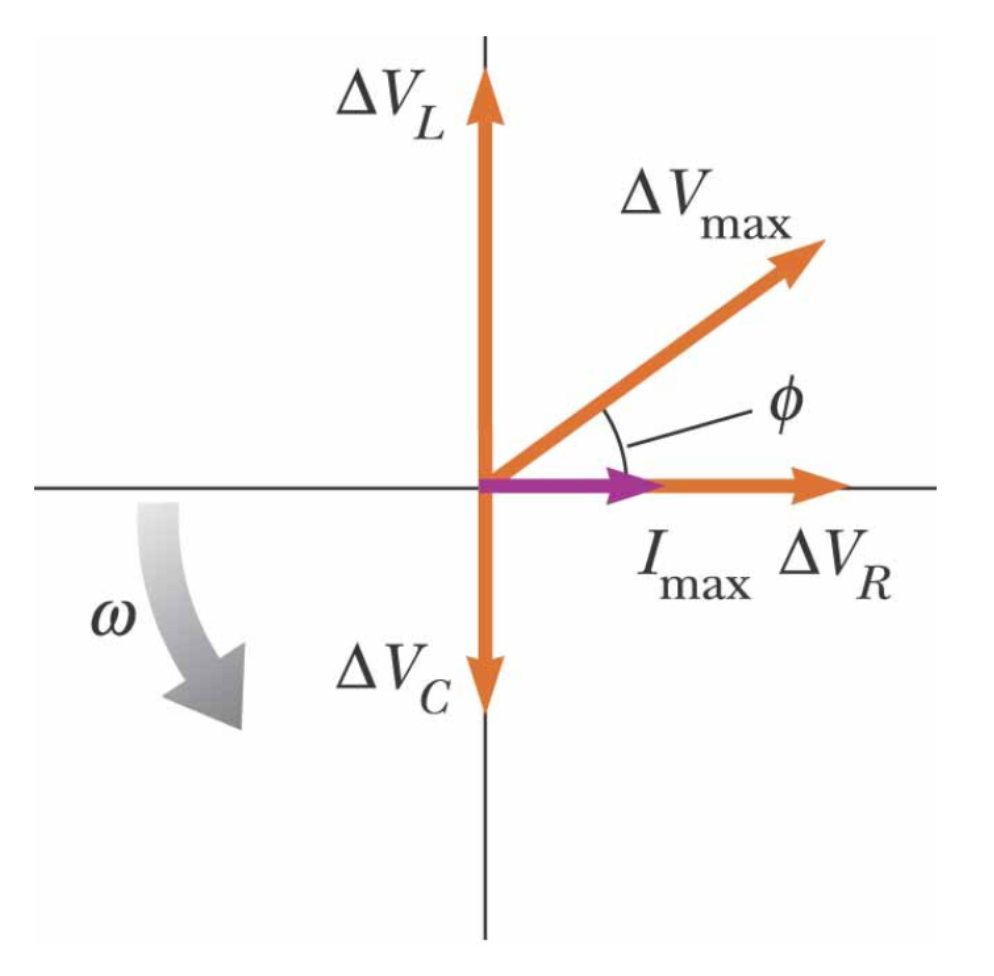
\includegraphics[scale = 0.3]{oz09/resources/Oef1Fasor.png}
        \end{center}
        waarbij $phi$ dient gezien te worden als een hoek van $20^\circ$.
\end{description}

\vspace{1cm}